\documentclass{article}

\usepackage{graphicx} % Required for inserting images
\usepackage{cmap} % поиск в PDF
\usepackage{amsthm, amssymb, amsfonts}
\usepackage{mathtext} % русские буквы в формулах
\usepackage[T2A]{fontenc} % кодировка
\usepackage[utf8]{inputenc} % кодировка
\usepackage[english,russian]{babel} % локализация и переносы
\usepackage{indentfirst}
\usepackage{amsmath}
\usepackage{mathtools}
\usepackage{tabto}

\begin{document}

\textbf{Задача 10.}
\textit{Стальная шаровая оболочка с внутренним радиусом 6 см
и внешним 10 см находится в стационарном тепловом состоянии.
Температура на внутренней ее поверхности равна $200^\circ$C,
а на внешней $20^\circ$C (рис. 7). Найти температуру на расстоянии
$r$ от центра и количество теплоты, которое в 1 сек шар отдает наружу
(теплопроводность стали $k=0,14$).}

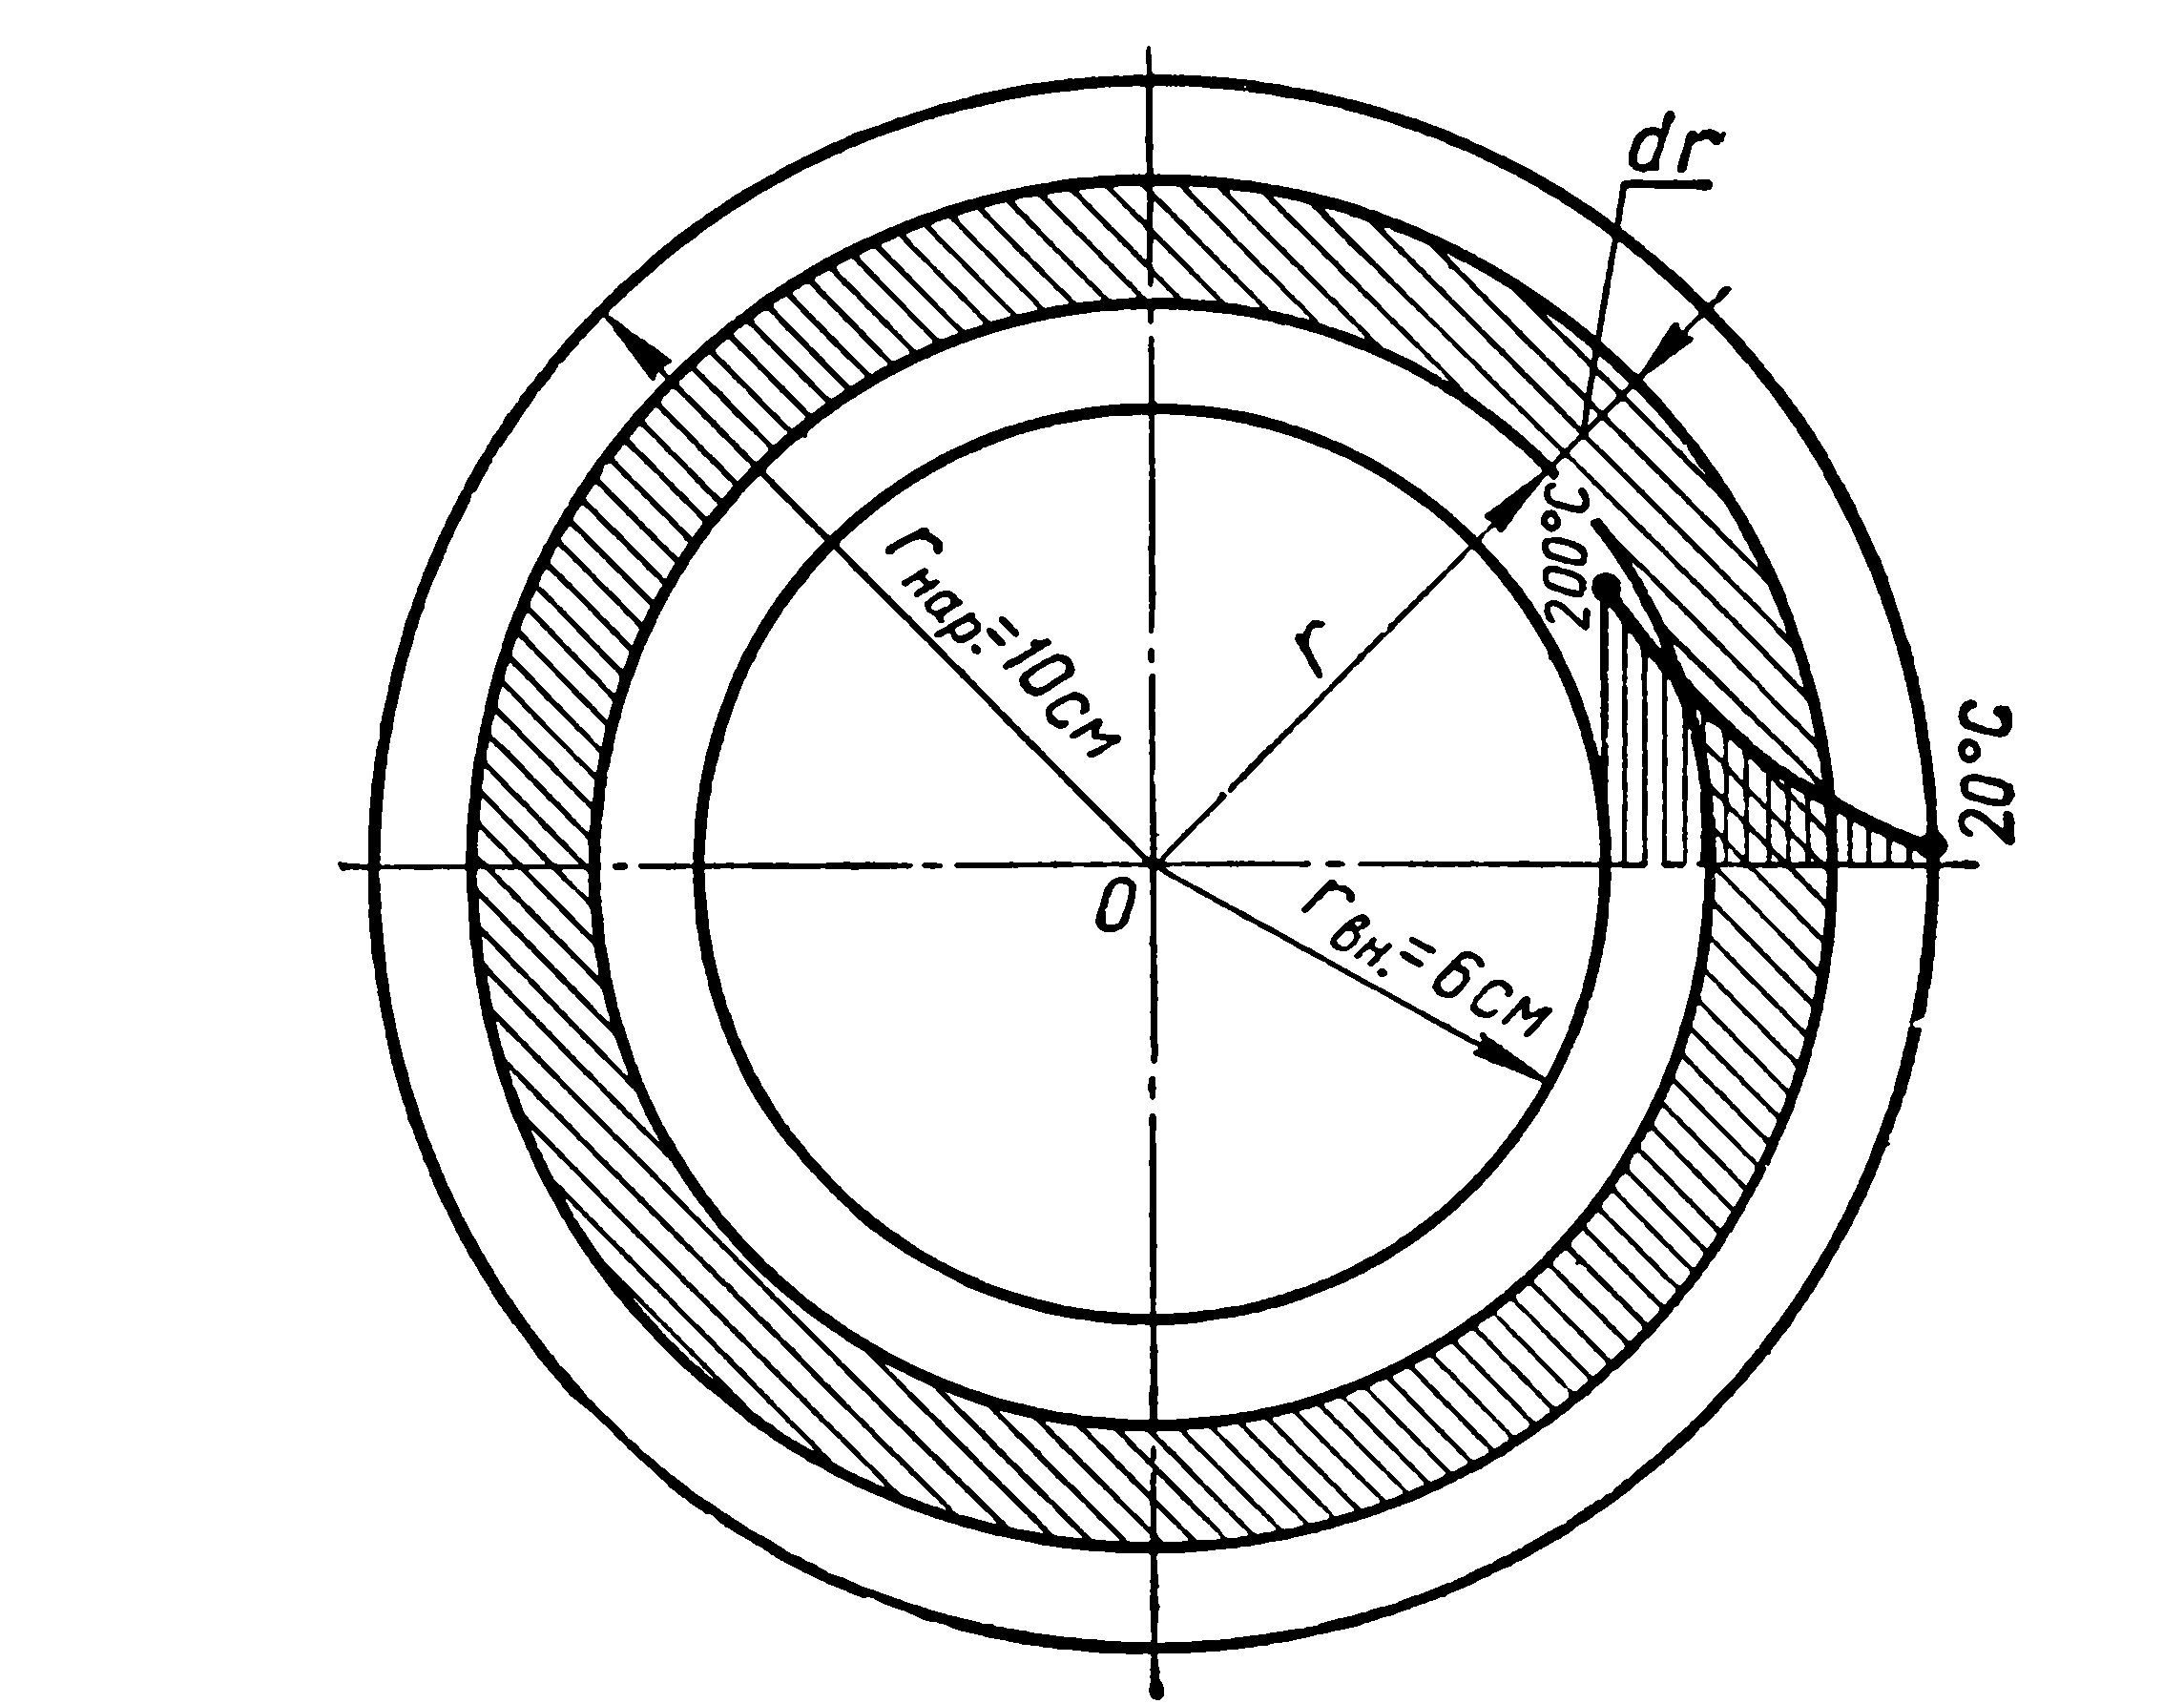
\includegraphics[width=4in]{./src/123.png}


\begin{center}
    \text{Решение}
\end{center}

На основании симметрии можно считать, что теплота в шаре
распространяется радиально. На расстоянии $r$ от центра площадь
протекания теплоты равна площади поверхности шара:

\begin{center}
    $F = 4\pi r^2$.
\end{center}

Ввиду того что между отдельными сферическими поверхностями
количество теплоты остается неизменным, через две любые поверхности
протекает одно и то же количество теплоты по закону теплопроводности
Фурье. Скорость, с которой теплота распространяется через площадку
$F$, равна:

\begin{center}
    $Q = -kF\frac{dT}{dr},$
\end{center}

\text{где $T$ --- температура тела,}

\text{$k$ --- теплопроводность вещества.}

\text{Уравнение (1) принимает вид:}

\begin{center}
    $-4\pi k r^2\frac{dT}{dr}=Q=\mathrm{const}.$
\end{center}

\text{Разделяя переменные и интегрируя, получаем общее решение задачи:}

\begin{center}
    $4\pi kT=\frac{Q}{r}+C.$
\end{center}

Для отыскания частного решения подставляем начальные условия
$T=20,\ r=10;\ T=200,\ r=6$ в уравнение (2) и определяем величины
$C$ и $Q$:

\[
\begin{cases}
80\pi k=\dfrac{Q}{10}+C,\\[6pt]
800\pi k=\dfrac{Q}{6}+C.
\end{cases}
\]

\text{Получаем:}

\begin{center}
    $C=-1000\pi k$
\end{center}

\text{и}

\begin{center}
    $Q=10800\pi k.$
\end{center}

\text{Таким образом, искомая температура на расстоянии $r$:}

\begin{center}
    $T=\dfrac{2700}{r}-250,$
\end{center}

\text{а количество теплоты, отдаваемое шаром в течение $1$ сек:}

\begin{center}
    $Q=10800\pi k=4750\ \text{кал.}$
\end{center}

\end{document}